\section{Task 6: Automated Parameter Tuning}

\subsection{Task Description}
The objective of this stage was to optimize the \texttt{LMR\_slope} (Late Move Reduction slope) parameter of the \texttt{SchachMaus} engine, assuming it to be within the interval $[0, 2]$. The other engine parameters were fixed to the suggested "reasonable" defaults: \texttt{NMP\_intercept} $= 3$, \texttt{NMP\_slope} $= 0$, \texttt{LMR\_intercept} $= 1$, \texttt{RFP\_intercept} $= -30$, and \texttt{RFP\_slope} $= 150$. We optimised for the time control of $30$ seconds$+0$.
\par In the language of Lecture 8, we need to optimize the function
\[
f: [0,2] \to \mathbb{R}, \quad f(x) = \text{Elo rating of engine with (LMR\_slope} = x\text{)}
\]
We can approximate the function $f$ by playing games between engines with varying $x$-parameters and using Task 1 to estimate the ratings. This yields evaluation data with noisy measurements, where the noise $\epsilon$ corresponds to the standard deviation of the posterior rating distribution obtained from Task 1. 

\subsection{How we did it}
We began by initialising five engine instances with \texttt{LMR\_slope} values $\{0, 0.5, 1.0, 1.5, 2.0\}$ and let them play a huge round-robin tournament. Each pair played 50 games (25 random positions $\times$ 2 colors) to establish a baseline rating.
\par From the initial results, we observed that engines with lower slopes performed significantly better than those with higher slopes. Intuitively, it seemed that aggressive move reduction caused the engine to miss critical tactical resources, and the "sweet spot" for compromising speed and performance might be somewhere between $0$ and $1$.
\par We then calculated the Gaussian Process with a Gaussian kernel as a surrogate model for $f$, using the built-in functionality of the DiceKriging-Package, heuristically setting an upper bound of $0.3$ for the length-scale parameter.
\par For the acquisition function, we calculate the Expected Improvement (EI) using the formula from Lecture 8. The plot below visualizes the GP fitted to the ratings of the initial five engines, which we approximated from the initial tournament results using Task 1. The blue line represents the GP mean prediction, and the shaded area is the $95\%$ confidence interval. The red line shows the Expected Improvement (scaled for visualization), indicating where the model suggests we should sample next.

\begin{figure}[H]
    \centering
    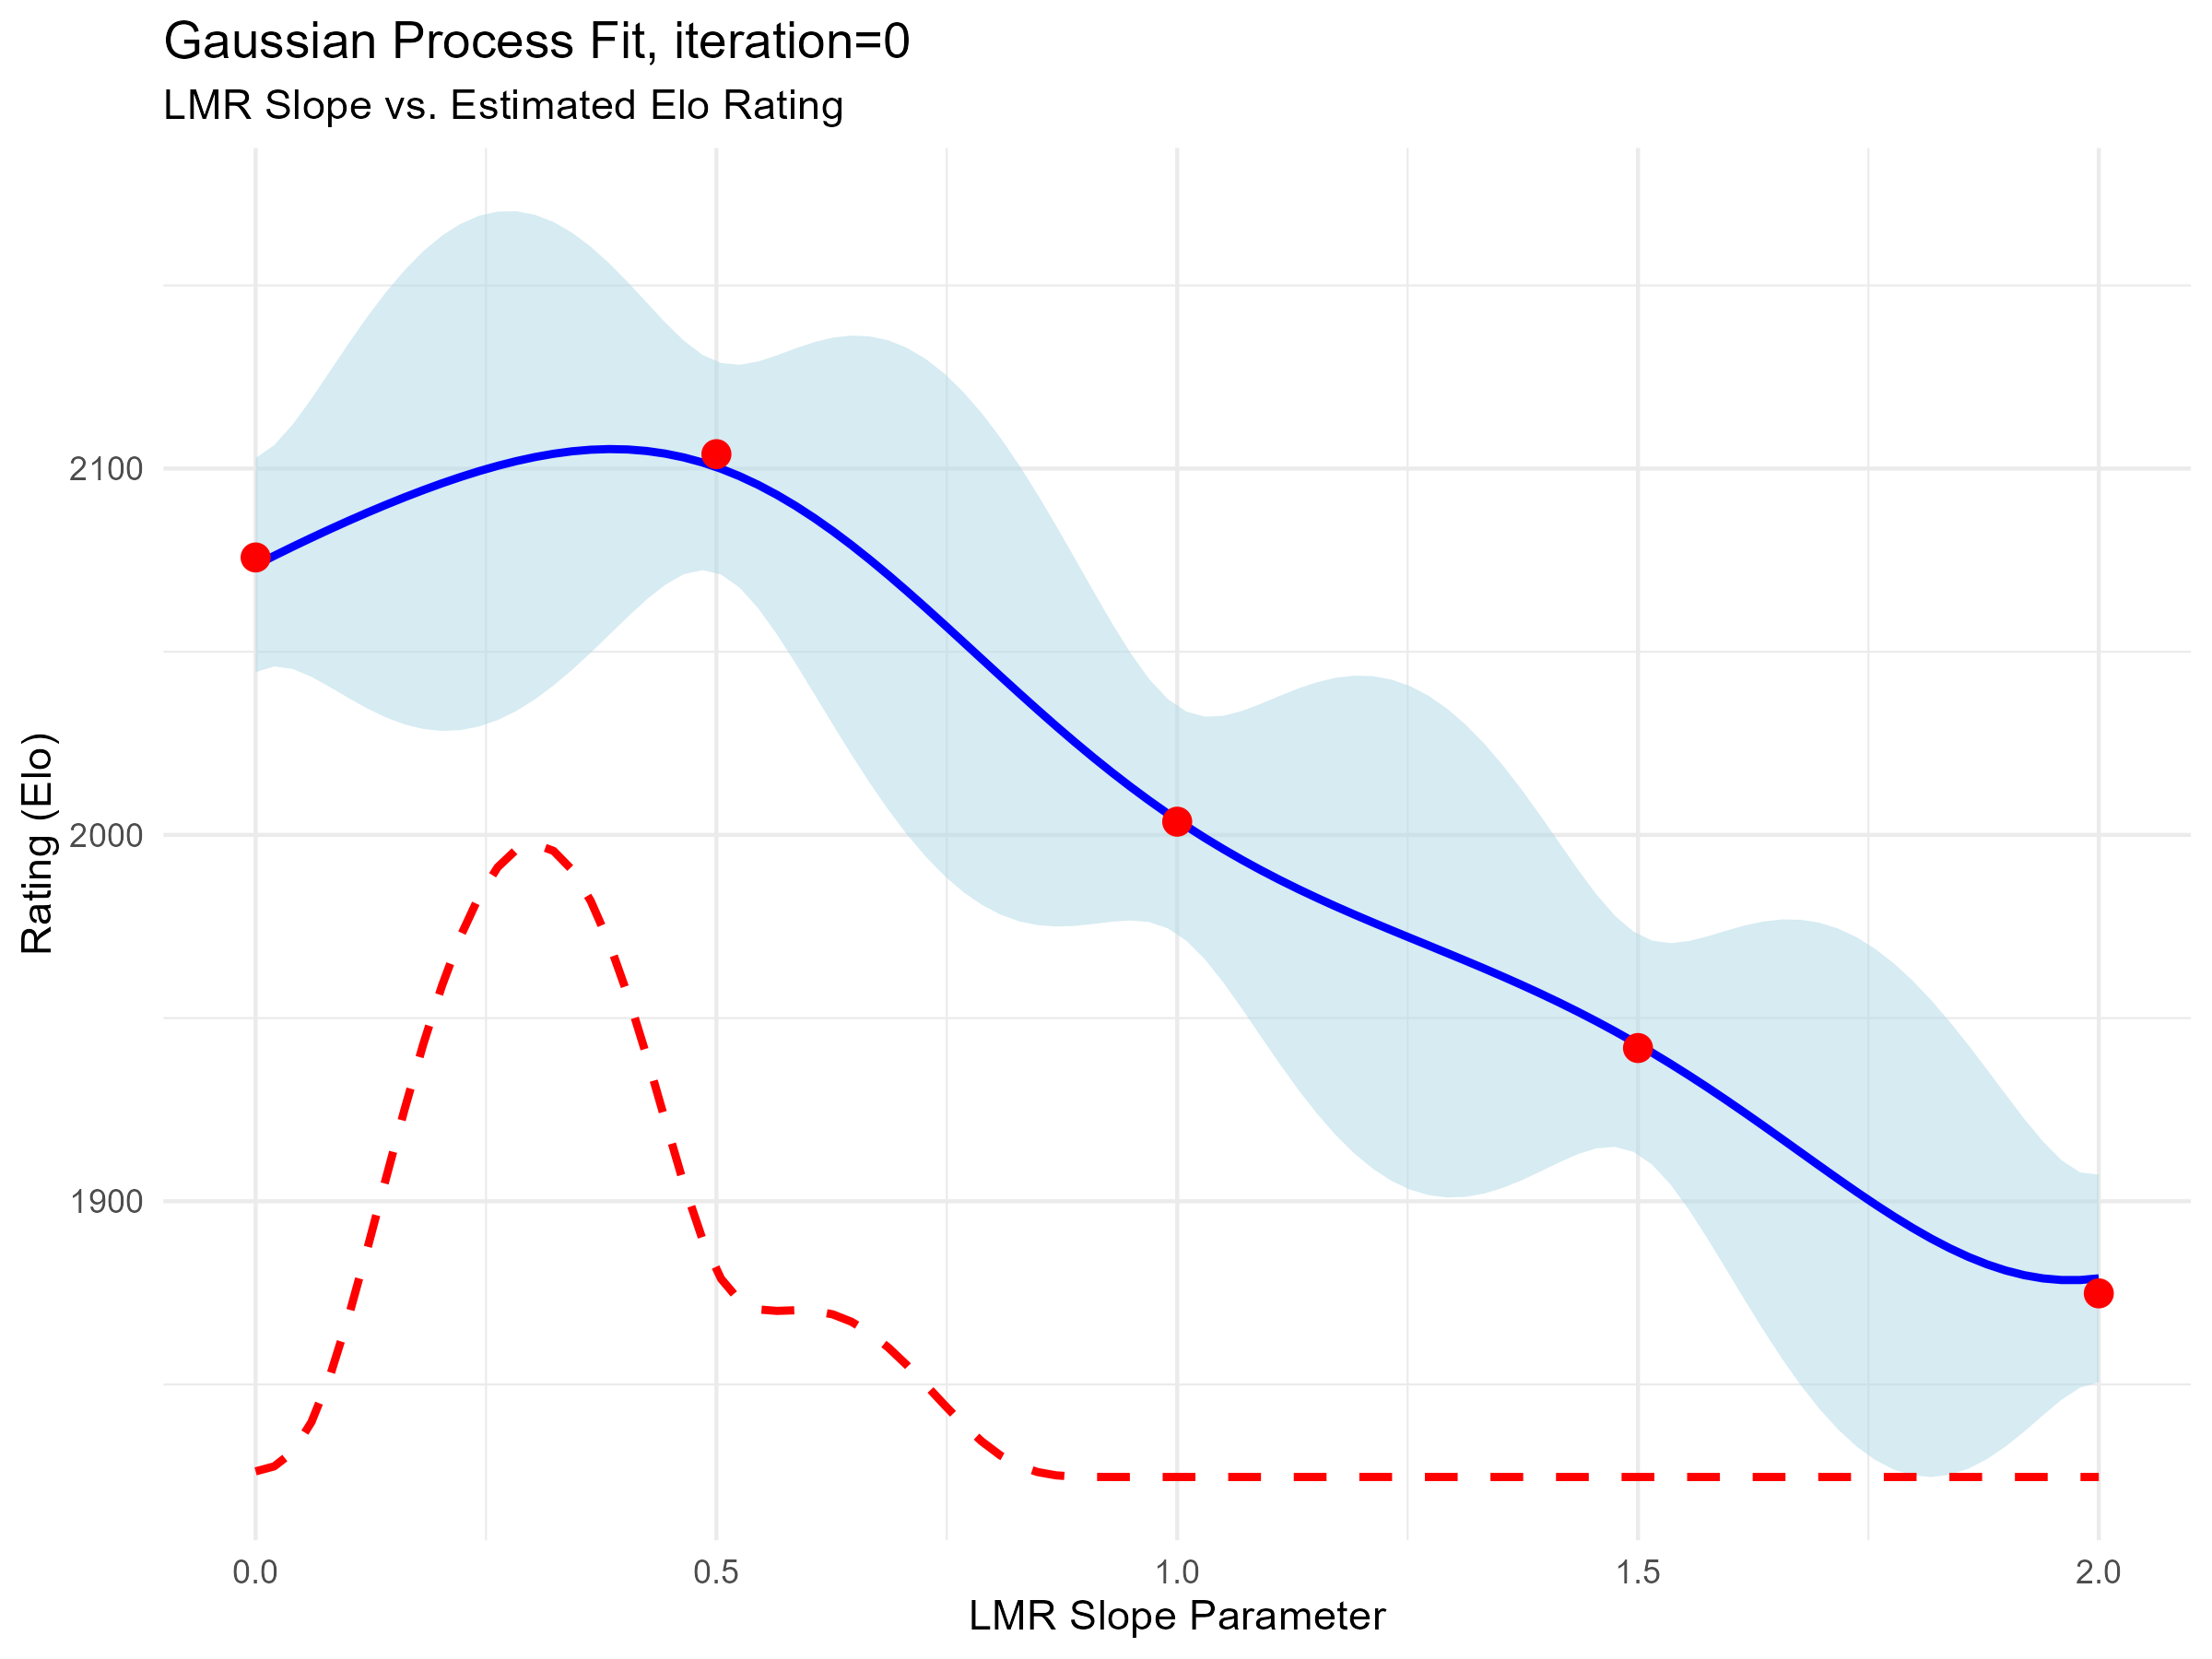
\includegraphics[width=0.8\textwidth]{media/initial_plot.png}
    \caption{Initial GP fit (Iteration 0) based on the 5 starting engines.}
    \label{fig:iter0}
\end{figure}

\par We then started the
\paragraph{Optimization Loop:}
\begin{enumerate}
    \item Maximize the EI function to identify the next candidate parameter and initialize a new engine with this parameter.
    \item Let the new engine play a mini-tournament against a diverse subset of existing engines: the current Best, 2nd Best, Median and Worst engines. A weighted round schedule (15, 10, 5, 2 games respectively) was used to prioritize comparison against the top engines. The weaker engines are included as further reference to the rating pool.
    \item Feed all results to the rating model from Task 1 to update the rating estimates for all engines, including the new one.
    \item Calculate the GP model with the new data points and plot it.
\end{enumerate}

\subsection{Results}
The optimization loop ran for 7 iterations. The GP quickly identified the optimal region to be in the lower range of the parameter space. The process terminated automatically during the 8th iteration, when the acquisition function suggested a parameter ($x=0.245$) that was identical to a previously tested value, because we had this as a termination condition in our optimization loop. In hindsight, since there are noisy measurements this termination condition does not make much sense.
\par The probability of improvement at the start of iteration 8 was $0.0360 (3.6\%)$. This is the final plot:
\begin{figure}[H]
    \centering
    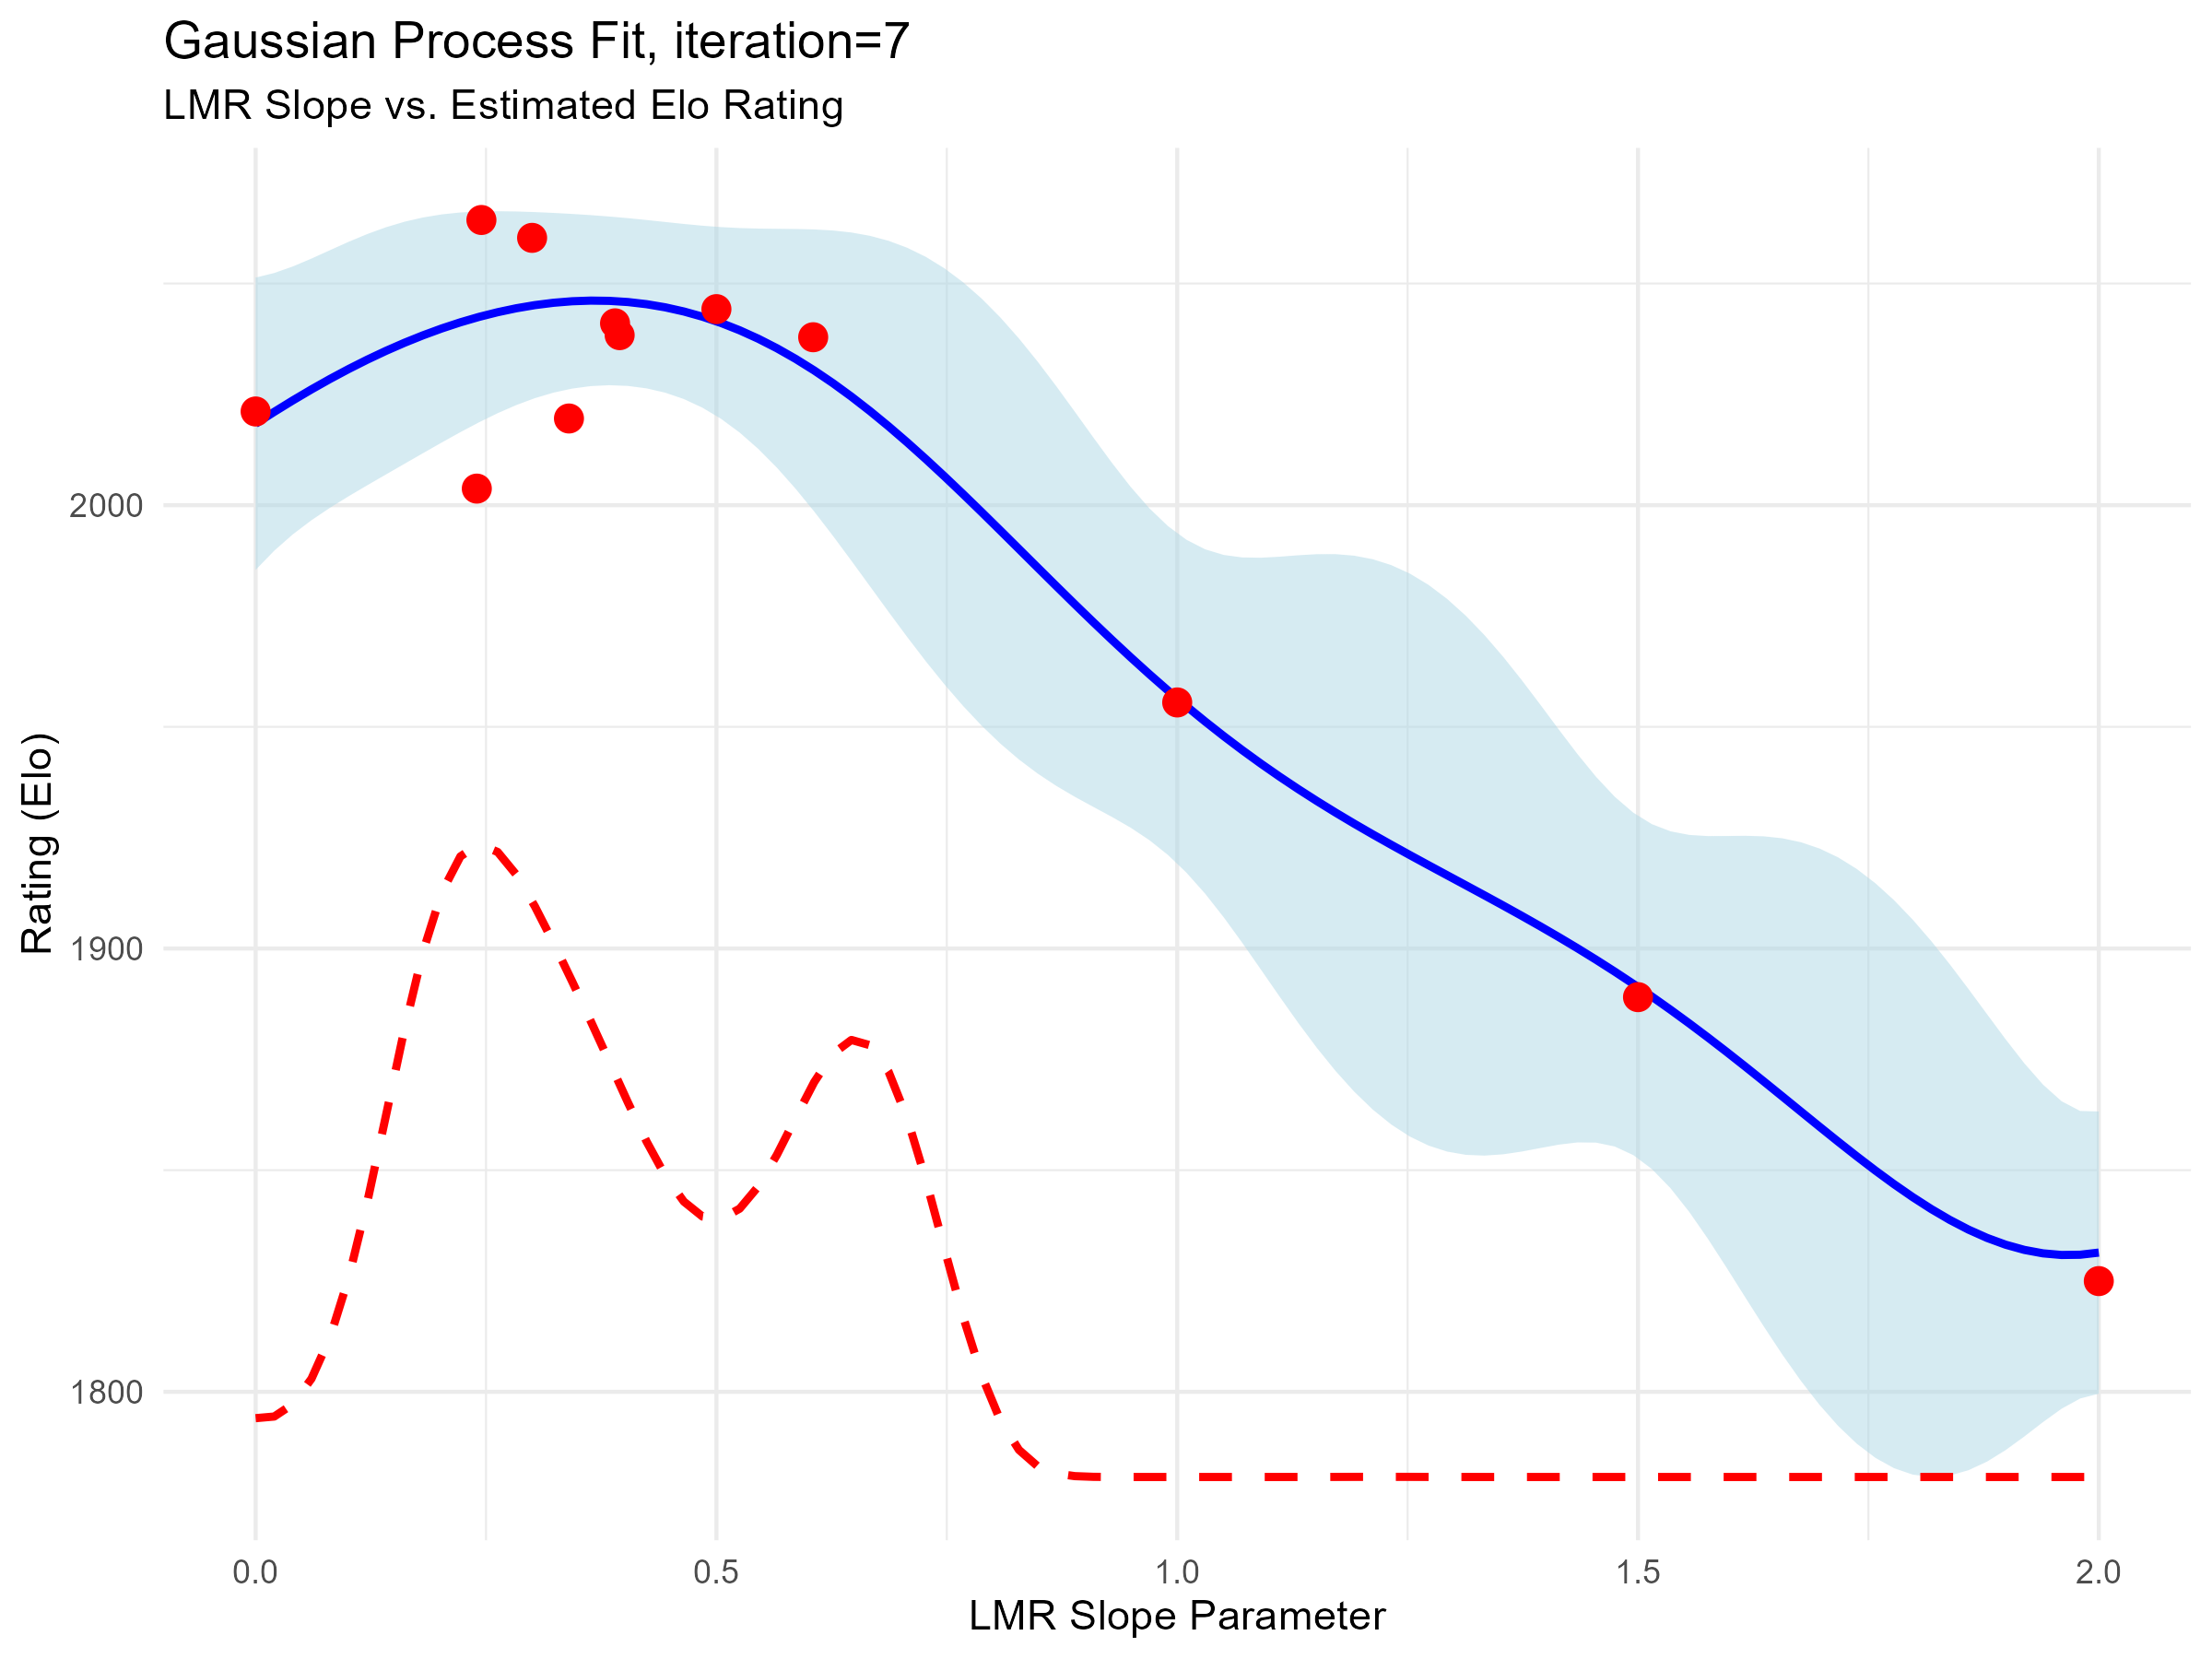
\includegraphics[width=0.8\textwidth]{media/optimization_iteration_7.png}
    \caption{Gaussian Process fit at Iteration 7.}
    \label{fig:optimization_process}
\end{figure}
\subsection{Conclusion}
Bayesian optimization identified an optimal \texttt{LMR\_slope} of $\approx 0.4$\footnote{There was a misunderstanding on our part here: of course, the "optimal" parameter should be taken as the maximum of the GP mean function, and not the next parameter selected by the EI function! Because we did not save the state of the variables and reproducing the results would take 8 hours of computing time letting the engines play games against each other, we can only approximate the optimal parameter from the plot.}.  An improvement to our code can be made when selecting the engines the new engine plays against in the optimization loop: Instead of choosing the median and the worst engine, select random engines instead. This way we get more "interesting" game results and prevent the phenomenon of certain engines who are not in contention for the nr. 1 spot playing much more games than the more relevant engines.